% !TeX root = ../thuthesis-example.tex

\chapter{求解方法与结果}

本章讨论含有混合整数追索的两阶段ARO的求解问题。混合整数追索问题由于其精确求解算法难以寻找,在许多以往的工作中在建模环节中被规避
,或采用适当的松弛与近似求解策略。然而,对于化工过程综合与优化问题,混合整数问题是广泛存在的,要求追索问题始终拥有连续的搜索空间,即第二阶段决策始终为连续变量会大大限制两阶段ARO在具体问题中的适用性与可解释性。因此,拓展混合整数追索的处理策略是一个ARO研究的关键问题。

\section{含有混合整数追索的两阶段ARO求解策略}
\label{section:solution}
首先,本文回顾在两阶段ARO问题的一般求解算法中获得成功的C\&CG算法流程并做适当讨论。

\subsection{列与约束生成算法}

列与约束生成算法(C\&CG)与传统的Benders分解方法不同,每次主问题-子问题迭代中,主问题都会增加一组追索变量,称为“列生成”(Column Generation),同时增加一项切平面约束。针对如式\eqref{eq:ccg1}--\eqref{eq:ccg2}的两阶段鲁棒优化问题:
\begin{align}
  \min_{\symbfit y}\quad &\symbfit c^T\symbfit y + \max_{\symbfit u\in\mathbb U} \min_{\symbfit x\in \mathit F(\symbfit y, \symbfit u)} \symbfit b^T \symbfit x \label{eq:ccg1}\\
   s.t.\ & \symbfit{Ay}\ge \symbfit a \\
   &  \symbfit G \symbfit x \ge \symbfit h - \symbfit E \symbfit y - \symbfit M \symbfit u\label{eq:ccg2}
\end{align}

原始的列与约束生成算法如算法\ref{alg:ccg}所示。
\label{section:ccg}

\begin{algorithm}
  \caption{求解\eqref{eq:ccg1}--\eqref{eq:ccg2}的C\&CG算法流程} \label{alg:ccg}
  \small
  \begin{algorithmic}
    \STATE{} 令 $LB=-\infty, UB=+\infty$ 和 $k = 0$
    \WHILE{TRUE}
    \STATE{} 求解下述主问题
    \begin{align}
      (\symbfup{MP})\min_{\symbfit{y,x},\eta}\quad & \symbfit c^T\symbfit y+\eta \\
      s.t.\ & \symbfit{Ay}\ge \symbfit a \\
      & \eta \ge \symbfit b^T\symbfit x^{l}, \forall 1\le l \le k \\
      & \symbfit G \symbfit x^l \ge \symbfit h - \symbfit E \symbfit y - \symbfit M \symbfit u_l^*, \forall 1\le l\le k \\
      &\symbfit y\in\mathbb Y, \symbfit x^l\in \mathbb X\subset\mathbb R_+^p\forall 1\le 1\le k
    \end{align}
    \STATE{} 获取最优解$(\symbfit y_{k+1}^*, \eta_{k+1}^*, \symbfit z^1, \dots, \symbfit z^k, \symbfit x^1, \dots, \symbfit x^k)$
    \STATE{} 更新$LB\leftarrow \symbfit c^T\symbfit y_{k+1}^*+\eta_{k+1}^*$
    \STATE{} 求解下列子问题
    \begin{align}
      (\symbfup{SP})& \mathcal{Q}(\hat{\symbfit y})=\max_{\symbfit u\in\mathbb U}\min_{x\in\mathbb X} \symbfit b^T\symbfit x \\
      s.t.\ & \symbfit G \symbfit x \ge \symbfit h - \symbfit E \symbfit{\hat{y}}  - \symbfit M \symbfit u
    \end{align}
    \STATE{} 更新$UB\leftarrow \min\{UB, \symbfit c^T\symbfit y_{k+1}^*+\mathcal Q(\symbfit y_{k+1}^*)\}$
      \IF{$UB-LB\le\varepsilon$}
        \STATE{} 当前$\symbfit y_{k+1}^*$为最优解,迭代终止。
      \ELSE[]
      \STATE{} 构造一列新变量$(\symbfit z^{k+1}, \symbfit x^{k+1})$,并向主问题增加下面各组约束:
      \begin{align}
        & \eta \ge \symbfit b^T\symbfit x^{k+1} \\
      & \symbfit G \symbfit x^{k+1} \ge \symbfit h - \symbfit E \symbfit y - \symbfit M \symbfit u_{k+1}^*, \forall 1\le l\le k \\
      &\symbfit y\in\mathbb Y, \symbfit x^l\in \mathbb X\subset\mathbb R_+^p\forall 1\le 1\le k
      \end{align}
      \STATE{} $k\leftarrow k+1$
      \ENDIF{}
    \ENDWHILE{}
  \end{algorithmic}
\end{algorithm}

上述算法比基于传统切平面的Benders分解方法在早期搜索阶段具有更高的计算效率\cite{zeng2013},因此现在被更广泛地应用于较大规模的ARO问题的精确求解。然而,上述流程对应用限制最严格的在于$\mathcal Q(\hat{\symbfit y})$的精确求解,对于$x\in\mathbb X\subset \mathbb R_+^p$的连续追索情形,用于在算法\ref{alg:ccg}中计算$\mathcal Q(\hat{\symbfit y})$的工具被称为“谕示机”(Oracle),通常是利用可调鲁棒对等问题的转化为可以通过其他梯度优化方法求取最优解的NLP子问题,因此,混合追索问题的谕示机的构造是富有挑战的。而且,对于常见的$\symbfit u\in\mathbb U$,在ARO问题迭代流程中主问题对应一个半无限规划问题,其收敛性的证明往往非常困难。所幸,列与约束生成算法在谕示机有能力寻找最差条件下的$\symbfit u^*$的前提下,其主问题上下界之间的收敛性已被证明\cite{zhao2011}。这启示我们将相应主问题的变量空间进行进一步分割,构造多层上下界以分别处理当前问题的混合追索问题。

\subsection{改进的三层问题求解流程}

参考\eqref{eq:ccg1}--\eqref{eq:ccg2}的形式,一般的含有整数追索的两阶段ARO可以表示为式\eqref{eq:miparo1}--\eqref{eq:miparo2}

\begin{align}
  \min_{\symbfit{y}\in\mathbb Y}\quad & \symbfit c^T\symbfit y+ \max_{\symbfit u\in\mathbb U}\min_{\symbfit{x,z}} \symbfit b^T\symbfit x + \symbfit d^T\symbfit z\label{eq:miparo1}\\
  s.t.\ & \symbfit{Ay}\ge \symbfit a \\
  & \symbfit G \symbfit x + \symbfit {Rz} \ge \symbfit h - \symbfit E \symbfit y - \symbfit M \symbfit u \\
  & \symbfit x\in \mathbb X\subset\mathbb R_+^p, \symbfit z\in\mathbb Z\subset\mathbb N_+^p \label{eq:miparo2}
\end{align}

在相关工作\cite{zhao2011,zeng2013,zhao2012}的启发下,我们假设整数追索变量$\symbfit z$是有界的。因此,$\symbfit z = \bigcup\{\symbfit z^r\}_{r=1}^{\mathcal R}$,其中$\mathcal R\le{\rm Card}(\{\symbfit z\in\mathbb N_+^p | \symbfup{dom\ \symbfit z}\})$,在这个前提下,\ref{section:ccg}节中算法\ref{alg:ccg}的子问题$(\symbfup{SP})$可以被转写为等价的有限约束数量的两层问题形式:

\begin{align}
  (\symbfup{SP^\prime})\ & \mathcal{Q}(\hat{\symbfit y})=\max \theta \\
  s.t.\ & \theta\le \symbfit d^T\symbfit z^r + \min_{\symbfit x^r\in\mathbb X}\{\symbfit b^T\symbfit x^r: \symbfit G \symbfit x^r +\symbfit R\symbfit z^r\ge \symbfit h - \symbfit E \symbfit{\hat{y}}  - \symbfit M \symbfit u \} \\& \forall 1\le r\le \mathcal R \\
  &\symbfit u\in\mathbb U
\end{align}

$\symbfup{SP^\prime}$可以通过KKT条件等价转化为单层形式:

\begin{align}
  (\symbfup{SP^\prime})\ & \mathcal{Q}(\hat{\symbfit y})=\max \theta \\
  s.t.\ & \theta\le \symbfit d^T\symbfit z^r + \symbfit b^T\symbfit x^r \\
  & \symbfit G \symbfit x^r +\symbfit R\symbfit z^r\ge \symbfit h - \symbfit E \symbfit{\hat{y}}  - \symbfit M \symbfit u, \forall 1\le r\le \mathcal R \\
  & \symbfit G^T\symbfit \pi^r \le \symbfit b, \forall 1\le r\le \mathcal R \\
  & \symbfit x^r(\symbfit G^T\symbfit \pi^r -\symbfit b) =0, \forall 1\le r\le \mathcal R\\
  & \symbfit \pi^r(\symbfit G \symbfit x^r +\symbfit R\symbfit z^r- \symbfit h +\symbfit E \symbfit{\hat{y}}+ \symbfit M \symbfit u) =0, \forall 1\le r\le \mathcal R \\ 
  &\symbfit u\in\mathbb U, \symbfit x^r\in\mathbb X\subset \mathbb R_+^p, \symbfit \pi^r\in\mathbb R_+^{p^\prime}, \forall 1\le r\le \mathcal R 
\end{align}

根据以上转化,我们可以采用单独的C\&CG算法循环来充当谕示机的作用。因此,本文建立的可以精确求解式\eqref{eq:miparo1}--\eqref{eq:miparo2}含有混合追索变量下子问题的$\mathcal Q(\hat{\symbfit y})$值的求解流程,如算法\ref{alg:nccg}所示。

\begin{algorithm}
  \caption{求解\eqref{eq:miparo1}--\eqref{eq:miparo2}的算法流程} \label{alg:nccg}
  \small
  \begin{algorithmic}
    \STATE{} 令 $LB=-\infty, UB=+\infty$ 和 $k = 0$
    \WHILE{TRUE}
    \STATE{} 求解下述主问题
    \begin{align}
      (\symbfup{MP})\min_{\symbfit{y,x},\eta}\quad & \symbfit c^T\symbfit y+\eta \\
      s.t.\ & \symbfit{Ay}\ge \symbfit a \\
      & \eta \ge \symbfit b^T\symbfit x^{l}, \forall 1\le l \le k \\
      & \symbfit G \symbfit x^l \ge \symbfit h - \symbfit E \symbfit y - \symbfit M \symbfit u_l^*, \forall 1\le l\le k \\
      &\symbfit y\in\mathbb Y, \symbfit x^l\in \mathbb X\subset\mathbb R_+^p\forall 1\le 1\le k
    \end{align}
    \STATE{} 获取最优解$(\symbfit y_{k+1}^*, \eta_{k+1}^*, \symbfit z^1, \dots, \symbfit z^k, \symbfit x^1, \dots, \symbfit x^k)$
    \STATE{} 更新$LB\leftarrow \symbfit c^T\symbfit y_{k+1}^*+\eta_{k+1}^*$
    \STATE{} 求解下列子问题
    \begin{align}
      (\symbfup{SP})& \mathcal{Q}(\hat{\symbfit y})=\max_{\symbfit u\in\mathbb U}\min_{x\in\mathbb X} \symbfit b^T\symbfit x \\
      s.t.\ & \symbfit G \symbfit x \ge \symbfit h - \symbfit E \symbfit{\hat{y}}  - \symbfit M \symbfit u
    \end{align}
    \STATE{} 更新$UB\leftarrow \min\{UB, \symbfit c^T\symbfit y_{k+1}^*+\mathcal Q(\symbfit y_{k+1}^*)\}$
      \IF{$UB-LB\le\varepsilon$}
        \STATE{} 当前$\symbfit y_{k+1}^*$为最优解,迭代终止。
      \ELSE[]
      \STATE{} 构造一列新变量$(\symbfit z^{k+1}, \symbfit x^{k+1})$,并向主问题增加下面各组约束:
      \begin{align}
        & \eta \ge \symbfit b^T\symbfit x^{k+1} \\
      & \symbfit G \symbfit x^{k+1} \ge \symbfit h - \symbfit E \symbfit y - \symbfit M \symbfit u_{k+1}^*, \forall 1\le l\le k \\
      &\symbfit y\in\mathbb Y, \symbfit x^l\in \mathbb X\subset\mathbb R_+^p\forall 1\le 1\le k
      \end{align}
      \STATE{} $k\leftarrow k+1$
      \ENDIF{}
    \ENDWHILE{}
  \end{algorithmic}
\end{algorithm}

\section{算例测试}

将算法\ref{alg:nccg}应用在一个含混合整数追索的两阶段ARO基准问题(Benchmarking Problem)中进行测试\cite{zhao2012}。考虑呼叫中心或诊所常见的员工轮岗排班问题(Rostering Problem),该优化问题要求要求在满足行业约束和服务需求的同时尽可能的降低运营成本。因此该案例考虑了两种类型的员工,分别为正式员工和兼职员工,兼职员工可以临时用来应对服务需求的波动变化,因此将兼职员工的安排问题设置为第二阶段决策问题。由此建立了一个两阶段可调的排班问题如下:

\begin{align}
  \min_{\symbfit x}\quad &\sum_i\sum_t c_{i,t}x_{i,t}+ \max_{\symbfit d}\min_{\symbfit{y,z,w}}\left(\sum_{j}\sum_t(f_{j,t}y_{j,t}+h_{j,t}z_{j,t})+\sum_tM_tw_t\right) \label{eq:roster1} \\
  s.t.\ & x_{i,t}+x_{i,t+1}+x_{i,t+2}\le 2, \forall i\le I, \forall t\le T-3 \label{eq:roster2}\\
  & l_i\le\sum_{t}x_{i,t}\le u_i, \forall i\le I \label{eq:roster3}\\
  & y_{j,t} + y_{j,t+1} \le 1, \forall j\le J, \forall t\le T-2 \label{eq:roster4}\\
  & a_j\le\sum_{t}y_{j,t}\le b_j, \forall j\le J \label{eq:roster5} \\
  & z_{j,t} \le Ny_{j,t}, \forall j\le J, \forall t\le T \label{eq:roster6} \\
  & N\sum_ix_{i,t}+\sum_{j}z_{j,t}+w_t\ge d_t, \forall t\le T \label{eq:roster7} \\
  & x_{i,t}, y_{j,t}\in\{0,1\}, z_{j,t}, w_t\ge0 \label{eq:roster8}
\end{align}

模型描述的问题背景较为显然,此处不再赘述。其中约束条件\eqref{eq:roster2}要求正式员工不能连续工作三个班次以上,式\eqref{eq:roster4}要求兼职员工不能连续工作两个班次以上,式\eqref{eq:roster3}和\eqref{eq:roster5}分别限制了正式员工和兼职员工调班次总数的上下限。式\eqref{eq:roster6}表示了兼职员工工作小时数的上限,式\eqref{eq:roster7}描述了工作需求与在班员工数量之间的约束关系,式\eqref{eq:roster8}定义了四个决策变量的取值范围。表\ref{tab:roster}中梳理了该模型中各参数和变量的含义,并对参数的取值或变量的类型做了说明。

\begin{longtable}{ccc}
    \caption{基准问题\eqref{eq:roster1}--\eqref{eq:roster8}中参数与变量符号释义及取值范围表}
    \label{tab:roster} \\
    \toprule
    参数 &  含义 & 取值范围\\
    \midrule
  \endfirsthead
    \caption*{续表~\thetable\quad 基准问题\eqref{eq:roster1}--\eqref{eq:roster8}中参数与变量符号释义及取值范围表} \\
    \toprule
    参数 &  含义 & 取值范围 \\
    \midrule
  \endhead
    \bottomrule
  \endfoot
  $c_{i,t}$ & 正式员工$i$的固定工资	& $[5,15]$中取固定值 \\
  $f_{j,t}$ & 兼职员工$j$的固定工资 & $[20,30]$中取固定值 \\	
  $h_{j,t}$ & 兼职员工$j$的每小时工资& $[4,8]$中取固定值 \\
  $M_t$ & 未满足的服务需求的单位惩罚成本	& $[40,50]$中取固定值\\
  $l_i$ &  正式员工$i$班次总数的下限  & $[4,8]$中取固定值 \\	
  $u_i$ &  正式员工$i$班次总数的上限& $[8,14]$中取固定值 \\
  $a_j$ &  兼职员工$j$班次总数的下限 & $[2,4]$中取固定值 \\	
  $b_j$ &  兼职员工$j$班次总数的上限 & $[4,6]$中取固定值\\	
  $N$ &  员工的最大工作小时数 &  $N=8$\\	
  $T$ &  模型考虑的班次总数  & $T=21$\\	
  $I$ &  正式员工的总人数   &  $I=12$\\	
  $J$ &  兼职员工的总人数	 &  $J=3$\\
  $x_{i,t}$ &  $t$班次内是否使用正式员工$i$ &	二元变量 \\
  $y_{j,t}$& $t$班次内是否使用兼职员工$j$	& 二元变量 \\
  $z_{j}$ & 兼职员工$j$的工作小时数	& 连续变量 \\
  $w_t$  & 未满足的服务需求小时数	& 连续变量 \\
  $d_t$  & 需求量	& 不确定性参数 \\
\end{longtable}

通过用Pyomo编程并通过GAMS调用CPLEX求解器求解这个该问题案例。原问题中包含316个整数二元决策变量,84个连续决策变量,609个约束条件和1个21维的不确定性参数集合。固定参数值采用随机选取的方法进行50次随机测试。合理设置模型的初始值,外层问题上下界迅速缩小,gap≤1\%左右时搜索较慢,但最终全部测试样例可以成功求解。图\ref{fig:roster}展示了在时的一次随机试验结果,此时,外层问题在迭代10次后模型的求解算法收敛到最优解。

\begin{figure}[ht!]
  \centering
  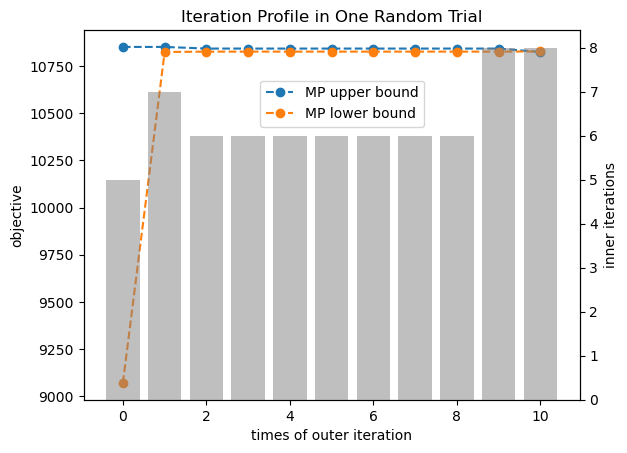
\includegraphics[width=0.8\linewidth]{roster.png}
  \caption{对算法\ref{alg:nccg}的某次基准问题测试收敛过程示意图}
  \label{fig:roster}
\end{figure}

因此,该求解流程可以有效求解一般的含有混合整数追索问题的ARO问题。

\section{本文不确定模型的求解}

本文的卢非酰胺连续合成超结构优化所建立的两阶段ARO模型适用于\ref{alg:nccg}的求解,具体转化与求解步骤见附录。下面着重探讨求解的结果。

\subsection{求解结果与分析}

本节中对模型\eqref{eq:aromodel1}-\eqref{eq:aromodel2}的求解采用GAMS 34.2.0编写程序并用BARON求解器\cite{kilinc2018}求解,计算所用个人电脑的配置资源如下:处理器型号Intel® CoreTM i7-10175H(基准速度2.59GHz), 内存16GB,采用全部线程求解。

经过计算得到的最优设计方案如表\ref{tab:rufiaro}所示。反应筛选到的最优设计路径方案为2-6-9,如图\ref{fig:rufiaro}所示。在三个反应步骤所设计采用的反应设备数量分别为7个、2个、4个,与确定性模型发生了较大的变化,另外,设计方案的最优目标函数为$1.198\times10^7$美元/年,相比确定性模型的结果提高了$53.3\%$左右,这是由于应对不确定性带来的成本提高,如预期生产规模的扩大、总时间上限的缩短和公用工程购买费用的提高。

\begin{table}[ht!]
  \centering
  \begin{threeparttable}[c]
    \caption{卢非酰胺连续合成超结构ARO模型优化结果}
    \label{tab:rufiaro}
    \begin{tabular}{cccccc}
      \toprule
       & 路径 & 设备需求量$\symbfit N_s$ & 总产量($\symbfit X_s$/mol) & 总产能(kg)& 目标函数值(美元/年) \\
      \midrule
      步骤一 & 2   &  7   &  557.61	 &  115.43   &  \multirow[c]{3}{*}{$1.198\times 10^7$} \\
      步骤二 & 6   &  2   &  557.56	 &  94.28   & \\
      步骤三 & 9   &  4  &  529.68	 &  150.00  & \\
      \bottomrule
    \end{tabular}
  \end{threeparttable}
\end{table}

\begin{figure}
  \centering
  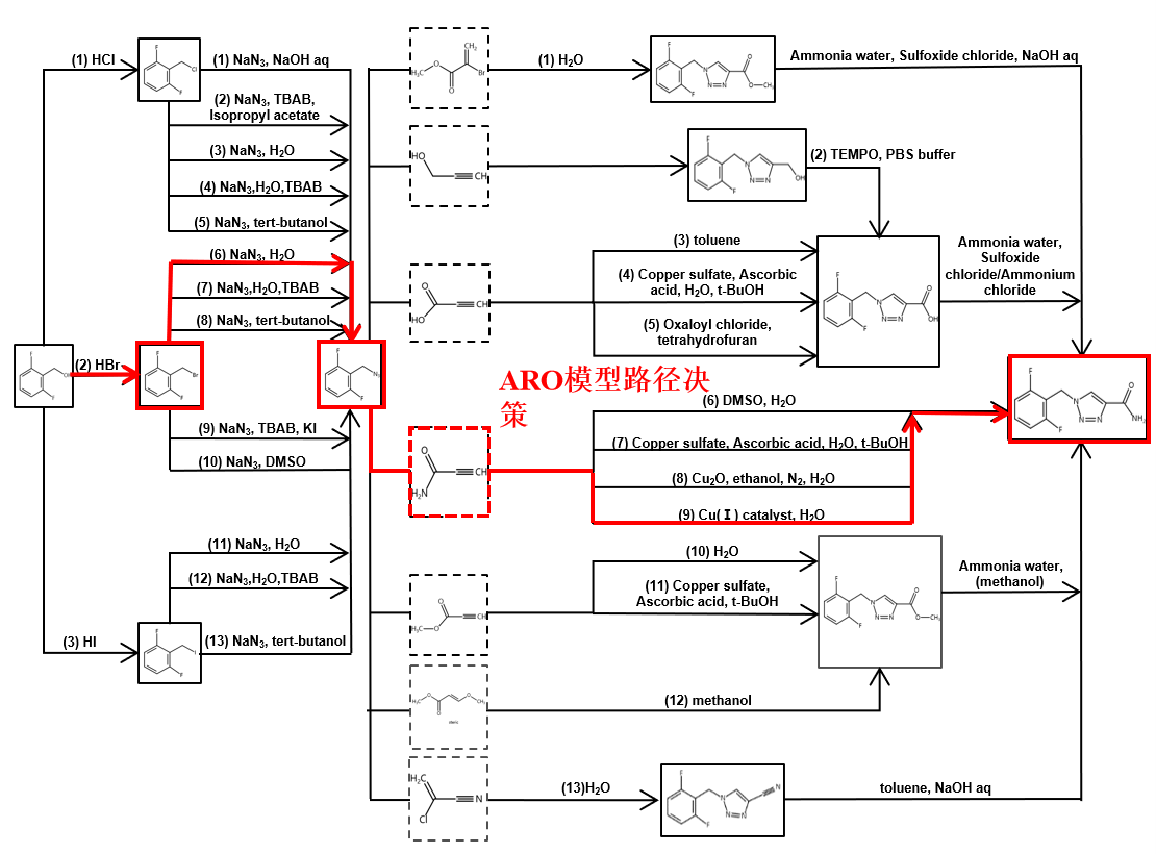
\includegraphics[width=1.1\linewidth]{ARO.png}
  \caption{ARO模型最优超结构路径选择图示}
  \label{fig:rufiaro}
\end{figure}

\subsection{不确定条件下的最优路径}

与确定性优化相比,ARO模型优化获得的求解路径发生改变,具体而言在本问题的模型中第三阶段的最优工艺路径选择发生改变。这说明在超结构优化中考虑不确定性参数的设计可能与不考虑不确定参数时拥有本质的不同,应对不确定性波动的能力更优的方案选择与在标称点下进行优化的最优方案选择不总是相同,这为决策者提供了另一种视角:过程抵抗不确定性波动的潜力与过程设计的预期成本之间存在一种博弈关系(Trade-off),决策者在概念设计阶段理性选择寻找二者之间的平衡点,是确定性模型与不确定性模型之间在模型解释性、参数响应性与最优决策的差异比较的关键作用。
在比较不确定性和确定性模型选出的最佳路径时,第一阶段和第二阶段得到的路径一致。然而,在第三阶段,不确定性模型选出了需要催化剂的路径9,而确定性模型则选出了成本更低的路径6,因为它不需要催化剂且原材料更经济。尽管如此,路径6在性能上不足以应对不确定性带来的挑战,这导致需要使用昂贵的一价铜催化剂来补偿。铜催化的叠氮-炔环加成反应是点击化学中一个典型例子,由诺贝尔奖得主K. Barry Sharpless提出,特点是高收率、广泛的应用、单一的副产物、立体选择性以及易于操作和溶剂去除。特别是,这个反应的速率比非催化的1,3-偶极环加成反应快100多倍。实验数据表明,在Cu(I)催化剂和水的体系下,卢非酰胺的一锅法合成过程可以达到95\%的最终收率,该结果说明了针对点击化学反应的研究与改进对高附加值化学品连续合成的工艺优化具有重要的潜在积极影响。

\subsection{鲁棒性检验}

本节对三种不确定性因素进行随机采样,随机选取50个不同的生产场景,讨论确定性优化方案和不确定性自适应可调鲁棒优化方案的样本外鲁棒性能。图\ref{fig:rotest}给出了确定性优化拓扑结构(2-6-6)和ARO优化拓扑结构(2-6-9)在上述50个场景下的成本效应。对比结果表明,两阶段ARO优化解析的拓扑结构能够以更低的成本应对随机场景,实现了鲁棒性能和经济性能更好的平衡。

\begin{figure}
  \centering
  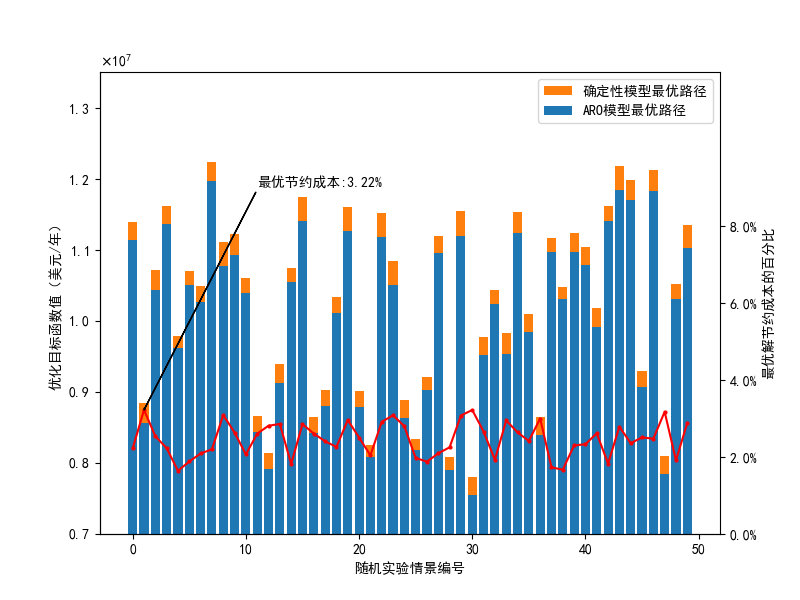
\includegraphics[width=\linewidth]{rotest.png}
  \caption{固定路径决策的确定性模型与ARO模型的随机试验目标函数对比}
  \label{fig:rotest}
\end{figure}



% % \section{数学符号}

% 中文论文的数学符号默认遵循 GB/T 3102.11—1993《物理科学和技术中使用的数学符号》
% \footnote{原 GB 3102.11—1993,自 2017 年 3 月 23 日起,该标准转为推荐性标准。}。
% 该标准参照采纳 ISO 31-11:1992 \footnote{目前已更新为 ISO 80000-2:2019。},
% 但是与 \TeX{} 默认的美国数学学会(AMS)的符号习惯有所区别。
% 具体地来说主要有以下差异:
% \begin{enumerate}
%   \item 大写希腊字母默认为斜体,如
%     \begin{equation*}
%       \Gamma \Delta \Theta \Lambda \Xi \Pi \Sigma \Upsilon \Phi \Psi \Omega.
%     \end{equation*}
%     注意有限增量符号 $\increment$ 固定使用正体,模板提供了 \cs{increment} 命令。
%   \item 小于等于号和大于等于号使用倾斜的字形 $\le$、$\ge$。
%   \item 积分号使用正体,比如 $\int$、$\oint$。
%   \item
%     偏微分符号 $\partial$ 使用正体。
%   \item
%     省略号 \cs{dots} 按照中文的习惯固定居中,比如
%     \begin{equation*}
%       1, 2, \dots, n \quad 1 + 2 + \dots + n.
%     \end{equation*}
%   \item
%     实部 $\Re$ 和虚部 $\Im$ 的字体使用罗马体。
% \end{enumerate}

% 以上数学符号样式的差异可以在模板中统一设置。
% 另外国标还有一些与 AMS 不同的符号使用习惯,需要用户在写作时进行处理:
% \begin{enumerate}
%   \item 数学常数和特殊函数名用正体,如
%     \begin{equation*}
%       \uppi = 3.14\dots; \quad
%       \symup{i}^2 = -1; \quad
%       \symup{e} = \lim_{n \to \infty} \left( 1 + \frac{1}{n} \right)^n.
%     \end{equation*}
%   \item 微分号使用正体,比如 $\dif y / \dif x$。
%   \item 向量、矩阵和张量用粗斜体(\cs{symbf}),如 $\symbf{x}$、$\symbf{\Sigma}$、$\symbfsf{T}$。
%   \item 自然对数用 $\ln x$ 不用 $\log x$。
% \end{enumerate}


% 英文论文的数学符号使用 \TeX{} 默认的样式。
% 如果有必要,也可以通过设置 \verb|math-style| 选择数学符号样式。

% 关于量和单位推荐使用
% \href{http://mirrors.ctan.org/macros/latex/contrib/siunitx/siunitx.pdf}{\pkg{siunitx}}
% 宏包,
% 可以方便地处理希腊字母以及数字与单位之间的空白,
% 比如:
% \SI{6.4e6}{m},
% \SI{9}{\micro\meter},
% \si{kg.m.s^{-1}},
% \SIrange{10}{20}{\degreeCelsius}。



% % \section{数学公式}

% 数学公式可以使用 \env{equation} 和 \env{equation*} 环境。
% 注意数学公式的引用应前后带括号,通常使用 \cs{eqref} 命令,比如式\eqref{eq:example}。
% \begin{equation}
%   \frac{1}{2 \uppi \symup{i}} \int_\gamma f = \sum_{k=1}^m n(\gamma; a_k) \mathscr{R}(f; a_k).
%   \label{eq:example}
% \end{equation}

% 多行公式尽可能在“=”处对齐,推荐使用 \env{align} 环境。
% \begin{align}
%   a & = b + c + d + e \\
%     & = f + g
% \end{align}



% % \section{数学定理}

% 定理环境的格式可以使用 \pkg{amsthm} 或者 \pkg{ntheorem} 宏包配置。
% 用户在导言区载入这两者之一后,模板会自动配置 \env{theorem}、\env{proof} 等环境。

% \begin{theorem}[Lindeberg--Lévy 中心极限定理]
%   设随机变量 $X_1, X_2, \dots, X_n$ 独立同分布, 且具有期望 $\mu$ 和有限的方差 $\sigma^2 \ne 0$,
%   记 $\bar{X}_n = \frac{1}{n} \sum_{i+1}^n X_i$,则
%   \begin{equation}
%     \lim_{n \to \infty} P \left(\frac{\sqrt{n} \left( \bar{X}_n - \mu \right)}{\sigma} \le z \right) = \Phi(z),
%   \end{equation}
%   其中 $\Phi(z)$ 是标准正态分布的分布函数。
% \end{theorem}
% \begin{proof}
%   Trivial.
% \end{proof}

% 同时模板还提供了 \env{assumption}、\env{definition}、\env{proposition}、
% \env{lemma}、\env{theorem}、\env{axiom}、\env{corollary}、\env{exercise}、
% \env{example}、\env{remar}、\env{problem}、\env{conjecture} 这些相关的环境。
